Input to the Streamflow Routing (SFR) Package is read from the file that has type ``SFR6'' in the Name File. Any number of SFR Packages can be specified for a single groundwater flow model; however, water cannot be routed between reaches in separate packages except in cases where the MVR Package is used to route water between separate packages.

Reach connectivity must be explicitly specified for this version of the SFR Package, unlike the abbreviated SFR Package segment connectivity specified in previous versions of MODFLOW. Explicit specification of reach connectivity has been adopted to facilitate better validation of stream network connectivity by the program. Explicit reach connectivity means that a reach must be specified as an upstream connection for all downstream connections to the reach. Downstream connections for a reach are denoted with a negative reach number. Flow in a reach is unidirectional, always flowing from the upstream end to the downstream end of a reach. An example of the reach connectivity for a hypothetical stream network is shown in figure~\ref{fig:sfr-connectivity}.

\begin{figure}[ht]
	\centering
	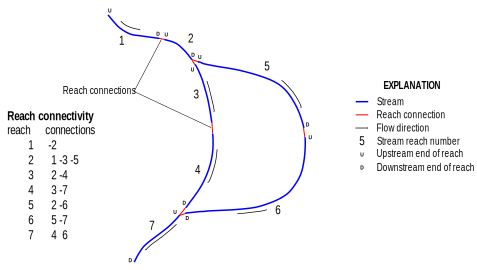
\includegraphics[scale=1.0]{../Figures/sfr-connectivity}
	\caption[Illustration of a simple stream network having seven reaches with a junction having two reaches, a confluence of two reaches, and the resulting reach connectivity]{Simple stream network having seven reaches with a junction having two reaches, a confluence of two reaches, and the resulting reach connectivity. Downstream connections for a reach must include the reach as an upstream connection for all downstream connections to the reach. Downstream connections for a  reach are denoted with a negative reach number}
	\label{fig:sfr-connectivity}
\end{figure}

Reaches can be specified to have a wide-rectangular cross-section or an irregular cross-section with an arbitrary number of station-elevation points (n-point cross-sections --- added in version 6.3.0). The approach used to represent n-point cross-sections in the SFR Package is a generalization of the 8-point cross-section available in the SFR Package for previous versions of MODFLOW \citep{modflowsfr1pack}. The station-elevation data for n-point cross-sections is specified as xfraction and depth data, which is converted to station position using the specified reach width and elevation using the specified top elevation of the reach stream bed. Fraction values were specified for the station data to maintain use of the specified reach width for reaches using n-point cross-sections. Furthermore, use of a maximum xfraction value less than or greater than one allows users to vary the width of a reach during a simulation.

Manning's roughness coefficient fractions can optionally be specified with the xfraction-depth data for a n-point cross-section to represent roughness coefficient variations in a channel (for example, different channel and overbank Manning's roughness coefficients). When Manning's coefficient fractions are specified, the streamflow is calculated for each segment of the n-point cross-section and summed to calculate the total streamflow for a reach; this is the same approach used in the SFR Package for previous versions of MODFLOW \citep{modflowsfr1pack} to calculate the stream flow for the left bank, defined channel, and right bank. Fraction values are specified for n-point cross-section Manning's roughness coefficient data in order to allow users to also set Manning's roughness coefficients in the stress period data and using timeseries.

\vspace{5mm}
\subsubsection{Structure of Blocks}

\vspace{5mm}
\noindent \textit{FOR EACH SIMULATION}
\lstinputlisting[style=blockdefinition]{./mf6ivar/tex/gwf-sfr-options.dat}
\lstinputlisting[style=blockdefinition]{./mf6ivar/tex/gwf-sfr-dimensions.dat}
\lstinputlisting[style=blockdefinition]{./mf6ivar/tex/gwf-sfr-packagedata.dat}

\vspace{5mm}
\noindent \textit{CROSSSECTIONS BLOCK IS OPTIONAL}
\lstinputlisting[style=blockdefinition]{./mf6ivar/tex/gwf-sfr-crosssections.dat}

\lstinputlisting[style=blockdefinition]{./mf6ivar/tex/gwf-sfr-connectiondata.dat}

\vspace{5mm}
\noindent \textit{IF ndv IS GREATER THAN ZERO FOR ANY REACH}
\lstinputlisting[style=blockdefinition]{./mf6ivar/tex/gwf-sfr-diversions.dat}

\vspace{5mm}
\noindent \textit{FOR ANY STRESS PERIOD}
\lstinputlisting[style=blockdefinition]{./mf6ivar/tex/gwf-sfr-period.dat}
\advancedpackageperioddescription{reach}{reaches}

\vspace{5mm}
\subsubsection{Explanation of Variables}
\begin{description}
% DO NOT MODIFY THIS FILE DIRECTLY.  IT IS CREATED BY mf6ivar.py 

\item \texttt{auxiliary}---defines an array of one or more auxiliary variable names.  There is no limit on the number of auxiliary variables that can be provided on this line; however, lists of information provided in subsequent blocks must have a column of data for each auxiliary variable name defined here.   The number of auxiliary variables detected on this line determines the value for naux.  Comments cannot be provided anywhere on this line as they will be interpreted as auxiliary variable names.  Auxiliary variables may not be used by the package, but they will be available for use by other parts of the program.  The program will terminate with an error if auxiliary variables are specified on more than one line in the options block.

\item \texttt{BOUNDNAMES}---keyword to indicate that boundary names may be provided with the list of stream reach cells.

\item \texttt{PRINT\_INPUT}---keyword to indicate that the list of stream reach information will be written to the listing file immediately after it is read.

\item \texttt{PRINT\_STAGE}---keyword to indicate that the list of stream reach stages will be printed to the listing file for every stress period in which ``HEAD PRINT'' is specified in Output Control.  If there is no Output Control option and \texttt{PRINT\_STAGE} is specified, then stages are printed for the last time step of each stress period.

\item \texttt{PRINT\_FLOWS}---keyword to indicate that the list of stream reach flow rates will be printed to the listing file for every stress period time step in which ``BUDGET PRINT'' is specified in Output Control.  If there is no Output Control option and \texttt{PRINT\_FLOWS} is specified, then flow rates are printed for the last time step of each stress period.

\item \texttt{SAVE\_FLOWS}---keyword to indicate that stream reach flow terms will be written to the file specified with ``BUDGET FILEOUT'' in Output Control.

\item \texttt{STAGE}---keyword to specify that record corresponds to stage.

\item \texttt{stagefile}---name of the binary output file to write stage information.

\item \texttt{BUDGET}---keyword to specify that record corresponds to the budget.

\item \texttt{FILEOUT}---keyword to specify that an output filename is expected next.

\item \texttt{budgetfile}---name of the binary output file to write budget information.

\item \texttt{TS6}---keyword to specify that record corresponds to a time-series file.

\item \texttt{FILEIN}---keyword to specify that an input filename is expected next.

\item \texttt{ts6\_filename}---defines a time-series file defining time series that can be used to assign time-varying values. See the ``Time-Variable Input'' section for instructions on using the time-series capability.

\item \texttt{OBS6}---keyword to specify that record corresponds to an observations file.

\item \texttt{obs6\_filename}---name of input file to define observations for the SFR package. See the ``Observation utility'' section for instructions for preparing observation input files. Table \ref{table:obstype} lists observation type(s) supported by the SFR package.

\item \texttt{MOVER}---keyword to indicate that this instance of the SFR Package can be used with the Water Mover (MVR) Package.  When the \texttt{MOVER} option is specified, additional memory is allocated within the package to store the available, provided, and received water.

\item \texttt{maximum\_iterations}---value that defines an maximum number of Streamflow Routing Newton-Raphson iterations allowed for a reach. By default, \texttt{maxsfrit} is equal to 100.

\item \texttt{maximum\_depth\_change}---value that defines the depth closure tolerance. By default, \texttt{dmaxchg} is equal to $1 \times 10^{-5}$.

\item \texttt{unit\_conversion}---value (or conversion factor) that is used in calculating stream depth for stream reach. A constant of 1.486 is used for flow units of cubic feet per second, and a constant of 1.0 is used for units of cubic meters per second. The constant must be multiplied by 86,400 when using time units of days in the simulation.

\item \texttt{maxbound}---integer value specifying the maximum number of stream reach cells that will be specified for use during any stress period.

\item \texttt{rno}---integer value that defines the reach number associated with the specified data on the line. \texttt{rno} must be greater than zero and less than or equal to \texttt{MAXBOUND}.

\item \texttt{cellid}---The keyword \texttt{`none'} must be specified for reaches that are not connected to an underlying GWF cell. The keyword \texttt{`none'} is used for reaches that are in cells that have \texttt{IDOMAIN} values less than one or are in areas not covered by the GWF model grid. Reach-aquifer flow is not calculated if the keyword \texttt{`none'} is specified.

\item \texttt{rlen}---real value that defines the reach length. \texttt{rlen} must be greater than zero.

\item \texttt{rwid}---real value that defines the reach width. \texttt{rwid} must be greater than zero.

\item \texttt{rgrd}---real value that defines the stream gradient (slope) across the reach. \texttt{rgrd} must be greater than zero.

\item \texttt{rtp}---real value that defines the top elevation of the reach streambed.

\item \texttt{rbth}---real value that defines the thickness of the reach streambed. \texttt{rbth} can be any value if \texttt{cellid} is \texttt{`none'}. Otherwise, \texttt{rbth} must be greater than zero.

\item \texttt{rhk}---real value that defines the hydraulic conductivity of the reach streambed. \texttt{rhk} can be any positive value if \texttt{cellid} is \texttt{`none'}. Otherwise, \texttt{rhk} must be greater than zero.

\item \textcolor{blue}{\texttt{man}---real or character value that defines the Manning's roughness coefficient for the reach. \texttt{man} must be greater than zero.  If the Options block includes a \texttt{TIMESERIESFILE} entry (see the ``Time-Variable Input'' section), values can be obtained from a time series by entering the time-series name in place of a numeric value.}

\item \texttt{ncon}---integer value that defines the number of reaches connected to the reach.

\item \texttt{ustrf}---real value that defines the fraction of upstream flow from each upstream reach that is applied as upstream inflow to the reach. The sum of all \texttt{ustrf} values for all reaches connected to the same upstream reach must be equal to one and \texttt{ustrf} must be greater than or equal to zero.

\item \texttt{ndv}---integer value that defines the number of downstream diversions for the reach.

\item \textcolor{blue}{\texttt{aux}---represents the values of the auxiliary variables for each stream reach. The values of auxiliary variables must be present for each stream reach. The values must be specified in the order of the auxiliary variables specified in the OPTIONS block.  If the package supports time series and the Options block includes a TIMESERIESFILE entry (see the ``Time-Variable Input'' section), values can be obtained from a time series by entering the time-series name in place of a numeric value.}

\item \texttt{boundname}---name of the stream reach cell.  \texttt{boundname} is an ASCII character variable that can contain as many as 40 characters.  If \texttt{boundname} contains spaces in it, then the entire name must be enclosed within single quotes.

\item \texttt{rno}---integer value that defines the reach number associated with the specified data on the line. \texttt{rno} must be greater than zero and less than or equal to \texttt{MAXBOUND}.

\item \texttt{ic}---integer value that defines the reach number of the reach connected to the current reach and whether it is connected to the upstream or downstream end of the reach. Negative \texttt{ic} numbers indicate connected reaches are connected to the downstream end of the current reach. Positive \texttt{ic} numbers indicate connected reaches are connected to the upstream end of the current reach. The absolute value of \texttt{ic} must be greater than zero and less than or equal to \texttt{MAXBOUND}.

\item \texttt{rno}---integer value that defines the reach number associated with the specified data on the line. \texttt{rno} must be greater than zero and less than or equal to \texttt{MAXBOUND}.

\item \texttt{idv}---integer value that defines the downstream diversion number for the diversion for reach \texttt{rno}. \texttt{idv} must be greater than zero and less than or equal to \texttt{ndv} for reach \texttt{rno}.

\item \texttt{iconr}---integer value that defines the downstream reach that will receive the diverted water. \texttt{idv} must be greater than zero and less than or equal to \texttt{MAXBOUND}. Furthermore, reach  \texttt{iconr} must be a downstream connection for reach \texttt{rno}.

\item \texttt{cprior}---character string value that defines the the prioritization system for the diversion, such as when insufficient water is available to meet all diversion stipulations, and is used in conjunction with the value of \texttt{flow} value specified in the \texttt{STRESS\_PERIOD\_DATA} section. Available diversion options include:  (1) \texttt{cprior} = `FRACTION', then the amount of the diversion is computed as a fraction of the streamflow leaving reach \texttt{rno} ($Q_{DS}$); in this case, 0.0 $\le$ \texttt{divflow} $\le$ 1.0.  (2) \texttt{cprior} = `EXCESS', a diversion is made only if $Q_{DS}$ for reach \texttt{rno} exceeds the value of \texttt{divflow}. If this occurs, then the quantity of water diverted is the excess flow ($Q_{DS} -$ \texttt{divflow}) and $Q_{DS}$ from reach \texttt{rno} is set equal to \texttt{divflow}. This represents a flood-control type of diversion, as described by Danskin and Hanson (2002). (3) \texttt{cprior} = `THRESHOLD', then if $Q_{DS}$ in reach \texttt{rno} is less than the specified diversion flow (\texttt{divflow}), no water is diverted from reach \texttt{rno}. If $Q_{DS}$ in reach \texttt{rno} is greater than or equal to (\texttt{divflow}), (\texttt{divflow}) is diverted and $Q_{DS}$ is set to the remainder ($Q_{DS} -$ \texttt{divflow})). This approach assumes that once flow in the stream is sufficiently low, diversions from the stream cease, and is the `priority' algorithm that originally was programmed into the STR1 Package (Prudic, 1989).  (4) \texttt{cprior} = `UPTO' -- if $Q_{DS}$ in reach \texttt{rno} is greater than or equal to the specified diversion flow (\texttt{divflow}), $Q_{DS}$ is reduced by \texttt{divflow}. If $Q_{DS}$ in reach \texttt{rno} is less than (\texttt{divflow}), \texttt{divflow} is set to $Q_{DS}$ and there will be no flow available for reaches connected to downstream end of reach \texttt{rno}.

\item \texttt{iper}---integer value specifying the starting stress period number for which the data specified in the PERIOD block apply.  \texttt{iper} must be less than \texttt{nper} in the TDIS Package and greater than zero.  The \texttt{iper} value assigned to a stress period block must be greater than the \texttt{iper} value assigned for the previous block.

\item \texttt{rno}---integer value that defines the reach number associated with the specified data on the line. \texttt{rno} must be greater than zero and less than or equal to \texttt{MAXBOUND}.

\item \texttt{sfrsetting}---line of information that is parsed into a keyword and values.  Keyword values that can be used to start the \texttt{sfrsetting} string include: \texttt{STATUS}, \texttt{MANNING}, \texttt{STAGE}, \texttt{INFLOW}, \texttt{RAINFALL}, \texttt{EVAPORATION}, \texttt{RUNOFF}, \texttt{DIVERSION}, \texttt{UPSTREAM\_FRACTION}, and \texttt{AUXILIARY}.

\begin{lstlisting}[style=blockdefinition]
STATUS <status>
MANNING <@manning@>
STAGE <@stage@>
INFLOW <@inflow@>
RAINFALL <@rainfall@>
EVAPORATION <@evaporation@>
RUNOFF <@runoff@>
DIVERSION <idv> <@divrate@> 
UPSTREAM_FRACTION <upstream_fraction>
AUXILIARY <auxname> <@auxval@> 
\end{lstlisting}

\item \texttt{status}---keyword option to define stream reach status.  \texttt{status} can be \texttt{ACTIVE}, \texttt{INACTIVE}, or \texttt{SIMPLE}. The \texttt{SIMPLE} \texttt{status} option simulates streamflow using a user-specified stage for a reach or a stage set to the top of the reach (depth = 0). In cases where the simulated leakage calculated using the specified stage exceeds the sum of inflows to the reach, the stage is set to the top of the reach and leakage is set equal to the sum of inflows. Upstream factions should be changed using the \texttt{UPSTREAM\_FRACTION} \texttt{sfrsetting} if the status for one or more reaches is changed to \texttt{ACTIVE} or \texttt{INACTIVE}. For example, if one of two downstream connections for a reach is inactivated, the upstream fraction for the active and inactive downstream reach should be changed to 1.0 and 0.0, respectively, to ensure that the active reach receives all of the downstream outflow from the upstream reach. By default, \texttt{status} is \texttt{ACTIVE}.

\item \textcolor{blue}{\texttt{manning}---real or character value that defines the Manning's roughness coefficient for the reach. \texttt{manning} must be greater than zero.  If the Options block includes a \texttt{TIMESERIESFILE} entry (see the ``Time-Variable Input'' section), values can be obtained from a time series by entering the time-series name in place of a numeric value.}

\item \textcolor{blue}{\texttt{stage}---real or character value that defines the stage for the reach. The specified \texttt{stage} is only applied if the reach uses the simple routing option. If \texttt{STAGE} is not specified for reaches that use the simple routing option, the specified stage is set to the top of the reach. If the Options block includes a \texttt{TIMESERIESFILE} entry (see the ``Time-Variable Input'' section), values can be obtained from a time series by entering the time-series name in place of a numeric value.}

\item \textcolor{blue}{\texttt{inflow}---real or character value that defines the volumetric inflow rate for the streamflow routing reach. If the Options block includes a TIMESERIESFILE entry (see the ``Time-Variable Input'' section), values can be obtained from a time series by entering the time-series name in place of a numeric value. By default, inflow rates are zero for each reach.}

\item \textcolor{blue}{\texttt{rainfall}---real or character value that defines the  volumetric rate per unit area of water added by precipitation directly on the streamflow routing reach. If the Options block includes a TIMESERIESFILE entry (see the ``Time-Variable Input'' section), values can be obtained from a time series by entering the time-series name in place of a numeric value. By default, rainfall  rates are zero for each reach.}

\item \textcolor{blue}{\texttt{evaporation}---real or character value that defines the  volumetric rate per unit area of water subtracted by evaporation from the streamflow routing reach. A positive evaporation rate should be provided. If the Options block includes a TIMESERIESFILE entry (see the ``Time-Variable Input'' section), values can be obtained from a time series by entering the time-series name in place of a numeric value. By default, evaporation rates are zero for each reach.}

\item \textcolor{blue}{\texttt{runoff}---real or character value that defines the volumetric rate of diffuse overland runoff that enters the streamflow routing reach. If the Options block includes a TIMESERIESFILE entry (see the ``Time-Variable Input'' section), values can be obtained from a time series by entering the time-series name in place of a numeric value. By default, runoff rates are zero for each reach.}

\item \texttt{DIVERSION}---keyword to indicate diversion record.

\item \texttt{idv}---diversion number.

\item \textcolor{blue}{\texttt{divrate}---real or character value that defines the volumetric diversion (\texttt{divflow}) rate for the streamflow routing reach. If the Options block includes a TIMESERIESFILE entry (see the ``Time-Variable Input'' section), values can be obtained from a time series by entering the time-series name in place of a numeric value.}

\item \texttt{upstream\_fraction}---real value that defines the fraction of upstream flow (\texttt{ustrf}) from each upstream reach that is applied as upstream inflow to the reach. The sum of all \texttt{ustrf} values for all reaches connected to the same upstream reach must be equal to one.

\item \texttt{AUXILIARY}---keyword for specifying auxiliary variable.

\item \texttt{auxname}---name for the auxiliary variable to be assigned \texttt{auxval}.  \texttt{auxname} must match one of the auxiliary variable names defined in the \texttt{OPTIONS} block. If \texttt{auxname} does not match one of the auxiliary variable names defined in the \texttt{OPTIONS} block the data are ignored.

\item \textcolor{blue}{\texttt{auxval}---value for the auxiliary variable.  If the Options block includes a TIMESERIESFILE entry (see the ``Time-Variable Input'' section), values can be obtained from a time series by entering the time-series name in place of a numeric value.}



\end{description}

\vspace{5mm}
\subsubsection{Example Input File}
\lstinputlisting[style=inputfile]{./mf6ivar/examples/gwf-sfr-example.dat}

\vspace{5mm}
\subsubsection{Available observation types}
Streamflow Routing Package observations include reach stage and all of the terms that contribute to the continuity equation for each stream reach. Additional SFR Package observations include the sum of inflows from upstream reaches and from mover terms (\texttt{upstream-flow}) and downstream outflow from a reach prior to diversions and the mover package (\texttt{downstream-flow}). The data required for each SFR Package observation type is defined in table~\ref{table:gwf-sfrobstype}. Negative and positive values for \texttt{sfr} observations represent a loss from and gain to the GWF model, respectively. For all other flow terms, negative and positive values represent a loss from and gain from the SFR package, respectively.

\FloatBarrier
\begin{longtable}{p{2cm} p{2.75cm} p{2cm} p{1.25cm} p{7cm}}
\caption{Available SFR Package observation types} \tabularnewline

\hline
\hline
\textbf{Stress Package} & \textbf{Observation type} & \textbf{ID} & \textbf{ID2} & \textbf{Description} \\
\hline
\endfirsthead

\captionsetup{textformat=simple}
\caption*{\textbf{Table \arabic{table}.}{\quad}Available SFR Package observation types.---Continued} \\

\hline
\hline
\textbf{Stress Package} & \textbf{Observation type} & \textbf{ID} & \textbf{ID2} & \textbf{Description} \\
\hline
\endhead


\hline
\endfoot

SFR & stage & rno or boundname & -- & Surface-water stage in a stream-reach boundary. If boundname is specified, boundname must be unique for each reach. \\
SFR & ext-inflow & rno or boundname & -- & Inflow into a stream-reach from an external boundary for a stream-reach or a group of stream-reaches. \\
SFR & inflow & rno or boundname & -- & Inflow into a stream-reach from upstream reaches for a stream-reach or a group of stream-reaches. \\
SFR & from-mvr & rno or boundname & -- & Inflow into a stream-reach from the MVR package for a stream-reach or a group of stream-reaches. \\
SFR & rainfall & rno or boundname & -- & Rainfall rate applied to a stream-reach or a group of stream-reaches. \\
SFR & runoff & rno or boundname & -- & Runoff rate applied to a stream-reach or a group of stream-reaches. \\
SFR & sfr & rno or boundname & -- & Simulated flow rate for a stream-reach and its aquifer connection for a stream-reach or a group of stream-reaches. \\
SFR & evaporation & rno or boundname & -- & Simulated evaporation rate from a stream-reach or a group of stream-reaches. \\
SFR & outflow & rno or boundname & -- & Outflow from a stream-reach to downstream reaches for a stream-reach or a group of stream-reaches. \\
SFR & ext-outflow & rno or boundname & -- & Outflow from a stream-reach to an external boundary for a stream-reach or a group of stream-reaches. \\
SFR & to-mvr & rno or boundname & -- & Outflow from a stream-reach that is available for the MVR package for a stream-reach or a group of stream-reaches. \\
SFR & upstream-flow & rno or boundname & -- & Upstream flow for a stream-reach or a group of stream-reaches from upstream reaches and the MVR package. \\
SFR & downstream-flow & rno or boundname & -- & Downstream flow for a stream-reach or a group of stream-reaches prior to diversions and the MVR package.

\label{table:gwf-sfrobstype}
\end{longtable}
\FloatBarrier

\vspace{5mm}
\subsubsection{Example Observation Input File}
\lstinputlisting[style=inputfile]{./mf6ivar/examples/gwf-sfr-example-obs.dat}

\newpage
\subsection{Streamflow Routing Package Cross-Sections Table Input File}
Cross-sections tables of distance fraction, depth, and optionally Manning's roughness coefficient fraction can be specified for individual reaches.  Cross-Section tables are specified by including file names in the CROSSSECTIONS or PERIOD blocks of the SFR Package.  These file names correspond to a Streamflow Routing cross-section table input file.  The format of the Streamflow Routing cross-section table input file is described here.

\vspace{5mm}
\subsubsection{Structure of Blocks}
\vspace{5mm}

\lstinputlisting[style=blockdefinition]{./mf6ivar/tex/utl-sfrtab-dimensions.dat}
\lstinputlisting[style=blockdefinition]{./mf6ivar/tex/utl-sfrtab-table.dat}
\vspace{5mm}

\vspace{5mm}
\subsubsection{Explanation of Variables}
\begin{description}
% DO NOT MODIFY THIS FILE DIRECTLY.  IT IS CREATED BY mf6ivar.py 

\item \textbf{Block: DIMENSIONS}

\begin{description}
\item \texttt{nrow}---integer value specifying the number of rows in the reach cross-section table. There must be NROW rows of data in the TABLE block.

\item \texttt{ncol}---integer value specifying the number of columns in the reach cross-section table. There must be NCOL columns of data in the TABLE block. Currently, NCOL must be equal to 2.

\end{description}
\item \textbf{Block: TABLE}

\begin{description}
\item \texttt{xfraction}---real value that defines the station (x) data for the cross-section as a fraction of the width (RWID) of the reach.

\item \texttt{depth}---real value that defines the elevation (z) data for the cross-section as a depth relative to the top elevation of the reach (RTP) and corresponding to the station data on the same line.

\end{description}


\end{description}

\subsubsection{Example Input File}
\lstinputlisting[style=inputfile]{./mf6ivar/examples/utl-sfrtab-example.dat}

